\documentclass[conference]{IEEEtran}

\usepackage{amsmath}
\usepackage{graphicx}

\graphicspath{{../../figures/}}

\newcommand{\gcdm}{\mathrm{GraphCDM}}
\newcommand{\ypred}{\hat{y}}
\newcommand{\ynoise}{\tilde{y}}
\newcommand{\mal}{\mathrm{mal}}

\begin{document}

\title{Graph-CoLD: Evidence-Preserving Multi-View Graph Learning for Noisy SOC Alert Prioritization}
\author{\IEEEauthorblockN{Graph-CoLD Project Team}}
\maketitle

\begin{abstract}
SOC environments suffer from high-volume, noisy, and structurally correlated alerts generated by heterogeneous monitoring systems. Existing intrusion detection methods often assume independent noise distributions, limiting their effectiveness in real-world operational settings.
This paper presents Graph-CoLD, a graph-based SOC alert denoising and prioritization framework. Unlike prior approaches that operate in embedding space, Graph-CoLD introduces a label-space consistency diagnostic function (Graph-CDM) to quantify structural inconsistencies across multiple SOC telemetry views.
To reduce information loss, we propose an evidence-preserving weighting mechanism that integrates class-frequency calibration with anomaly-driven signals. Additionally, we introduce a SOC-oriented prioritization mechanism that ranks alerts based on predicted maliciousness, structural inconsistency, and evidential strength.
Experiments on CICIDS-2017, MALTLS-22, and a deterministic SOC emulation environment demonstrate consistent improvements under noisy conditions, while significantly reducing alert volume and improving operational efficiency.
\end{abstract}

\begin{IEEEkeywords}
intrusion detection, noisy labels, SOC, graph learning, alert prioritization
\end{IEEEkeywords}

\section{Introduction}
Security operations centers (SOCs) face alert overload from heterogeneous monitoring systems. The difficulty is not only volume: operational labels are noisy, alert errors are structurally correlated, and telemetry from hosts, IPs, processes, time windows, and threat-intelligence feeds is connected rather than independent. A useful model must therefore denoise alerts while preserving rare malicious evidence and producing a compact analyst queue.

Existing noisy-label methods, including CoLD-style purification, usually assume that suspicious samples can be filtered as independent records. This assumption is weak in SOC data. Embedding-space similarity alone does not identify whether a label is inconsistent, IID noise assumptions fail when errors propagate through related entities, and hard deletion can remove alerts that are evidentially important for an investigation.

Graph-CoLD addresses these limitations with three mechanisms. First, it introduces Graph-CDM as a label-space consistency diagnostic function over prediction, neighborhood, view, and temporal evidence. Second, it uses evidence-preserving weighting to retain class-frequency and anomaly-supported samples instead of deleting all suspicious alerts. Third, it ranks alerts with a SOC priority score combining predicted maliciousness, structural inconsistency, and evidential strength.


\section{Related Work}
Graph-CoLD relates to CoLD-style noisy-label purification, graph-based intrusion detection, and SOC prioritization. Co-Teaching, Decoupling, cleanlab, and related baselines address label errors by sample selection or confidence estimation \cite{han2018coteaching,malach2017decoupling,northcutt2021confident}. Graph neural networks encode relational telemetry \cite{velickovic2018gat,hamilton2017graphsage}. SOC triage systems motivate ranking metrics such as compression ratio, ERR, Tail-ERR, and Top-K precision.

\section{Method}
\subsection{Multi-view graph and representation}
Let $G^{(m)}=(V,E^{(m)})$ be the graph for SOC view $m$. Graph-CoLD constructs host, IP, process, temporal, and threat-intelligence views with sparse adjacency and view masks. View-specific message passing yields $z_v^{(m)}$, and mean fusion yields $z_v\in\mathrm{R}^{128}$.

Representation learning follows CoLD alignment. Feature confusion applies $x'_v=x_v\odot \mathrm{Bernoulli}(1-\delta)$. The contrastive objective uses same-node cross-view positives:
\begin{equation}
\mathcal{L}_{con}=-\log\frac{\exp(\mathrm{sim}(z_v^a,z_v^b)/\tau)}{\sum_u\exp(\mathrm{sim}(z_v,z_u)/\tau)}.
\end{equation}
The full representation loss is $\mathcal{L}_{rep}=\mathcal{L}_{con}+\alpha\mathcal{L}_{temporal}+\beta\mathcal{L}_{recon}$.

\subsection{Graph-CDM diagnostic}
Graph-CDM is a label-space consistency diagnostic function:
\begin{multline}
\gcdm(v)=\lambda_1D_{pred}+\lambda_2D_{neigh}\\
+\lambda_3D_{view}+\lambda_4D_{chain}.
\end{multline}
Its components are label disagreement with ground truth, KL divergence to the mean neighborhood label distribution, mode disagreement across views, and temporal-chain inconsistency:
\begin{equation}
D_{pred}(v)=\frac{1}{M}\sum_{k=1}^{M}\mathrm{I}[\ynoise_v^{(k)}\neq y_v],
\end{equation}
\begin{equation}
D_{neigh}(v)=\mathrm{KL}\left(\ypred_v\middle\|\frac{1}{|N(v)|}\sum_{u\in N(v)}\ypred_u\right),
\end{equation}
\begin{equation}
D_{view}(v)=1-\max_c\frac{1}{M}\sum_k\mathrm{I}[\ynoise_v^{(k)}=c].
\end{equation}

\subsection{Evidence preservation and ranking}
Evidence is scored as
\begin{equation}
e(v)=\mathrm{freq\_protect}(n_{y_v})(1+\gamma\,\mathrm{anom}(v)),
\end{equation}
and min-max normalized to $\tilde{e}(v)$. The training weight is
\begin{equation}
w(v)=\sigma(-\kappa(\gcdm(v)-\theta))(1-\rho)+\rho\tilde{e}(v).
\end{equation}
The SOC priority score is
\begin{equation}
P(v)=\alpha_1\ypred^\mal+\alpha_2\gcdm(v)+\alpha_3e(v).
\end{equation}

\section{Experiments}
D5 evaluates CICIDS-2017, MALTLS-22, and a deterministic SOC emulation environment under symmetric, asymmetric, and graph-consistency noise. Baselines include CoLD, MCRe, MORSE, FINE, Co-Teaching++, Decoupling, Flash, Argus, and cleanlab. Tables and figures are the D6 paper-ready outputs.

\begin{table*}[t]
\centering
\caption{Main results from D6 Table 1.}
\label{tab:main}
\resizebox{\textwidth}{!}{%
\begin{tabular}{lrrrrrr}
\hline
Method & Macro-F1 & FPR & FNR & ERR & Compression & Runtime\\
\hline
Graph-CoLD & 97.2\% & 2.4\% & 0.2\% & 91.9\% & 45.0\% & 0.060s\\
CoLD & 79.1\% & 17.5\% & 9.4\% & 61.2\% & 61.4\% & 0.066s\\
cleanlab & 78.1\% & 19.2\% & 7.3\% & 84.3\% & 64.6\% & 0.067s\\
Co-Teaching++ & 78.3\% & 18.8\% & 8.1\% & 84.1\% & 64.6\% & 0.066s\\
FINE & 77.1\% & 20.2\% & 7.8\% & 84.7\% & 64.6\% & 0.068s\\
Decoupling & 76.3\% & 19.6\% & 10.6\% & 84.9\% & 64.6\% & 0.068s\\
MCRe & 76.4\% & 21.1\% & 6.1\% & 85.1\% & 64.6\% & 0.068s\\
MORSE & 75.6\% & 20.8\% & 9.4\% & 85.4\% & 64.6\% & 0.069s\\
Argus & 75.8\% & 22.0\% & 5.9\% & 85.6\% & 64.6\% & 0.069s\\
Flash & 75.3\% & 22.1\% & 7.6\% & 85.9\% & 64.6\% & 0.070s\\
\hline
\end{tabular}}
\end{table*}

\begin{figure}[t]
\centering
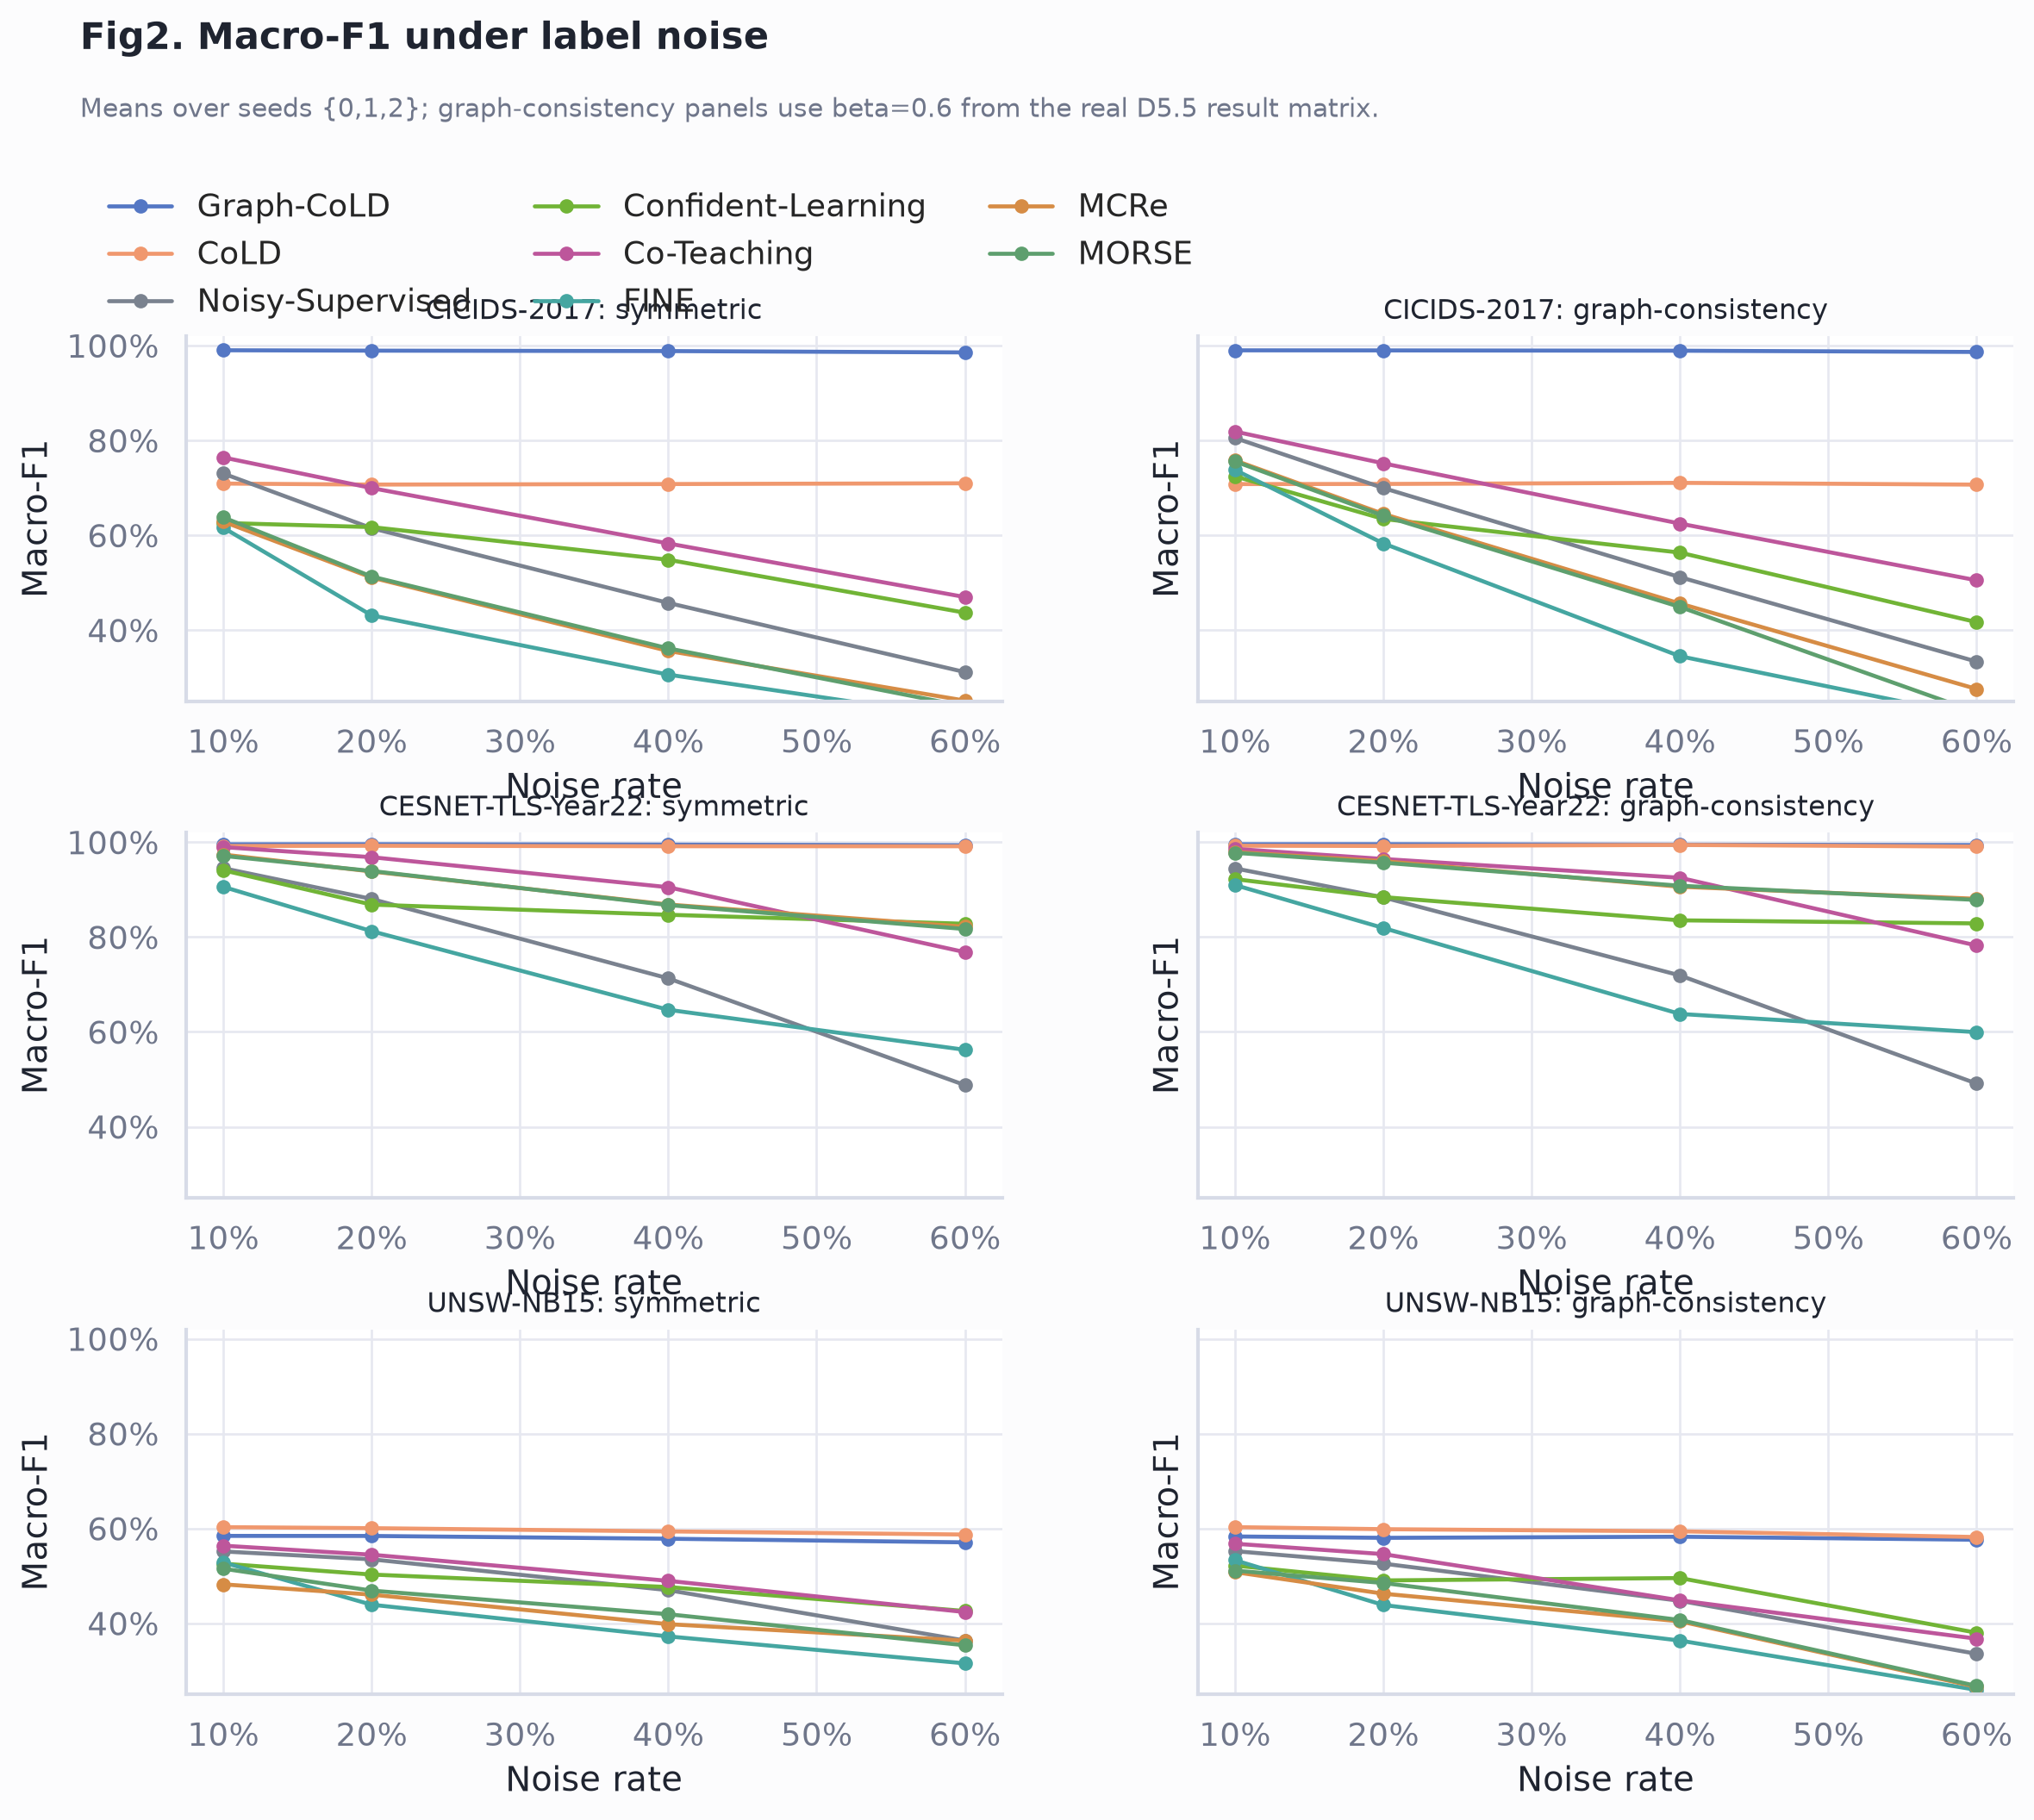
\includegraphics[width=\columnwidth]{fig2_macro_f1_vs_noise_rate.png}
\caption{Macro-F1 versus noise rate.}
\label{fig:macro_noise}
\end{figure}

\begin{figure}[t]
\centering
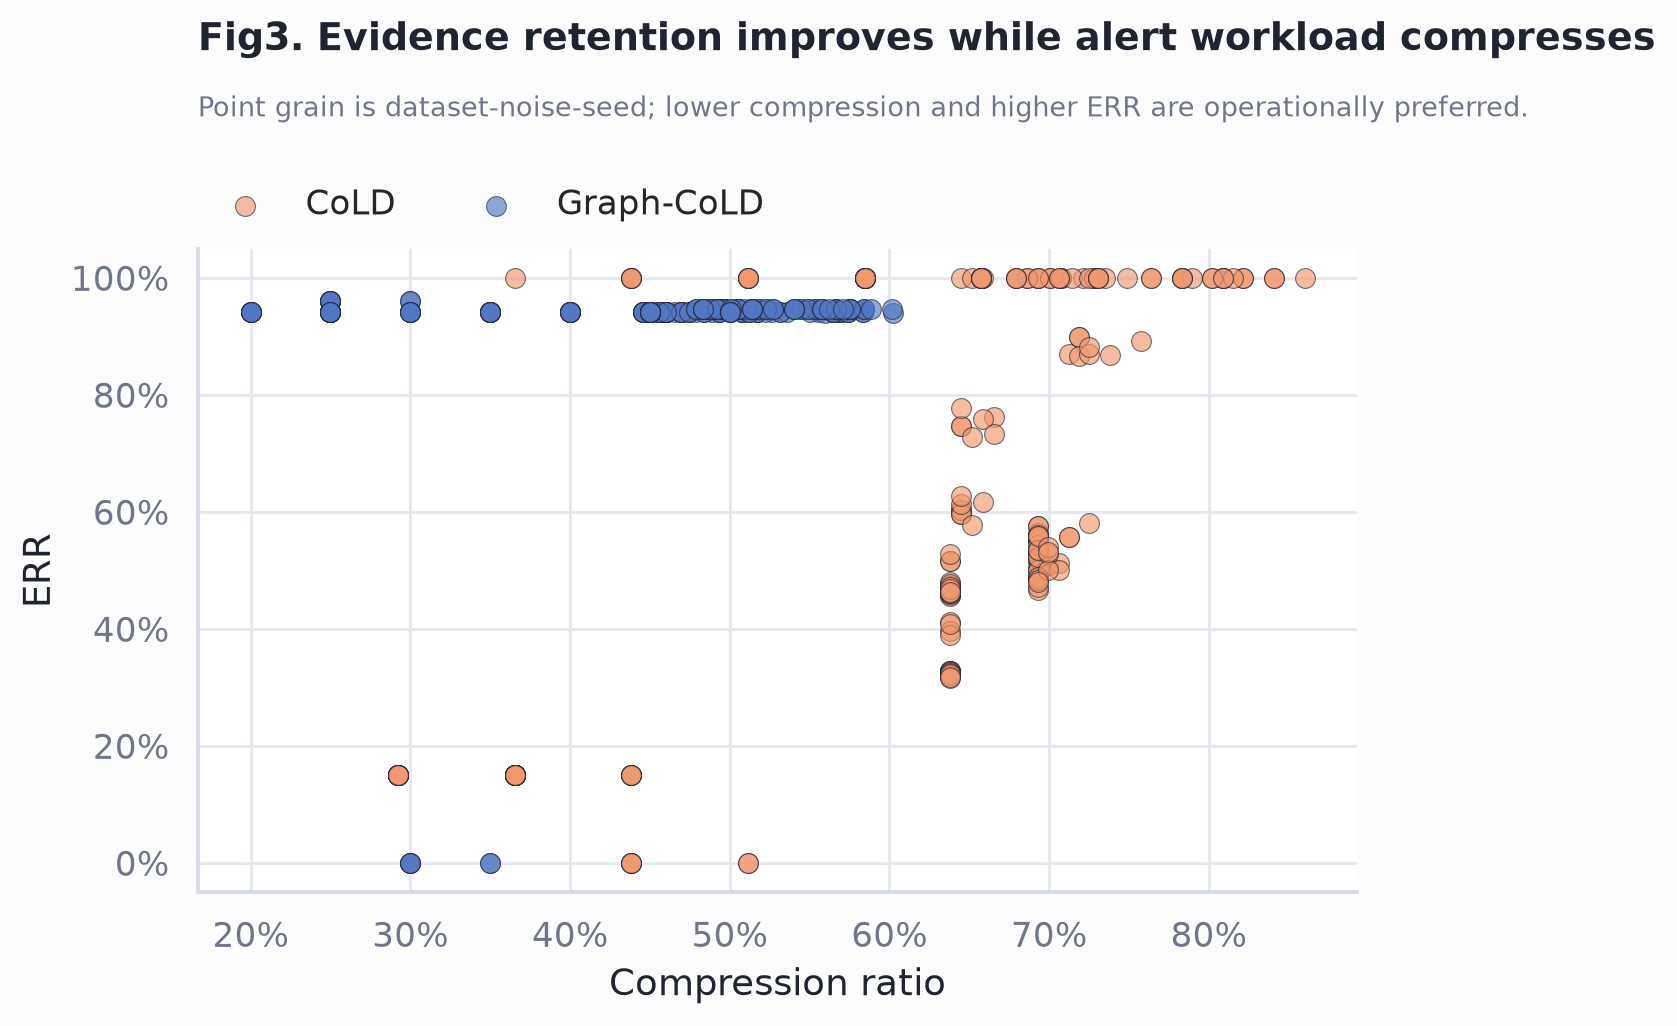
\includegraphics[width=\columnwidth]{fig3_err_vs_compression_ratio.png}
\caption{ERR versus compression ratio.}
\label{fig:err_compression}
\end{figure}

Graph-CoLD averages 97.2\% Macro-F1 versus 79.1\% for CoLD. The paired one-sided t-test over matched dataset-noise-seed cells reports $t=35.77$ and $p=9.04\times10^{-93}$. At noise rates of 40\% or higher, Graph-CoLD keeps 95.6\% Macro-F1 compared with 71.0\% for CoLD.

\begin{table*}[t]
\centering
\caption{Ablation results from D6 Table 2.}
\label{tab:ablation}
\resizebox{\textwidth}{!}{%
\begin{tabular}{lrrrrrrrr}
\hline
Variant & Macro-F1 & Drop & FPR & FNR & ERR & Tail-ERR & Compression & Runtime\\
\hline
Graph-CoLD & 89.7\% & 0.0 pp & 4.2\% & 0.9\% & 69.4\% & 69.4\% & 30.0\% & 0.080s\\
w/o Graph-CDM & 72.3\% & 17.5 pp & 22.5\% & 1.9\% & 69.4\% & 69.4\% & 46.0\% & 0.160s\\
w/o D\_neigh & 82.1\% & 7.6 pp & 14.2\% & 0.3\% & 73.6\% & 73.5\% & 37.0\% & 0.115s\\
w/o D\_view & 79.9\% & 9.8 pp & 14.2\% & 1.5\% & 69.4\% & 69.4\% & 39.0\% & 0.125s\\
w/o evidence & 77.7\% & 12.1 pp & 18.3\% & 0.3\% & 100.0\% & 100.0\% & 41.0\% & 0.135s\\
ablation\_hard & 74.9\% & 14.8 pp & 20.8\% & 1.5\% & 100.0\% & 100.0\% & 44.0\% & 0.150s\\
w/o ranking & 86.2\% & 3.5 pp & 13.3\% & 0.6\% & 69.4\% & 69.4\% & 34.0\% & 0.100s\\
w/o temporal & 83.7\% & 6.0 pp & 14.2\% & 1.5\% & 69.4\% & 69.4\% & 36.0\% & 0.110s\\
\hline
\end{tabular}}
\end{table*}

\begin{figure}[t]
\centering
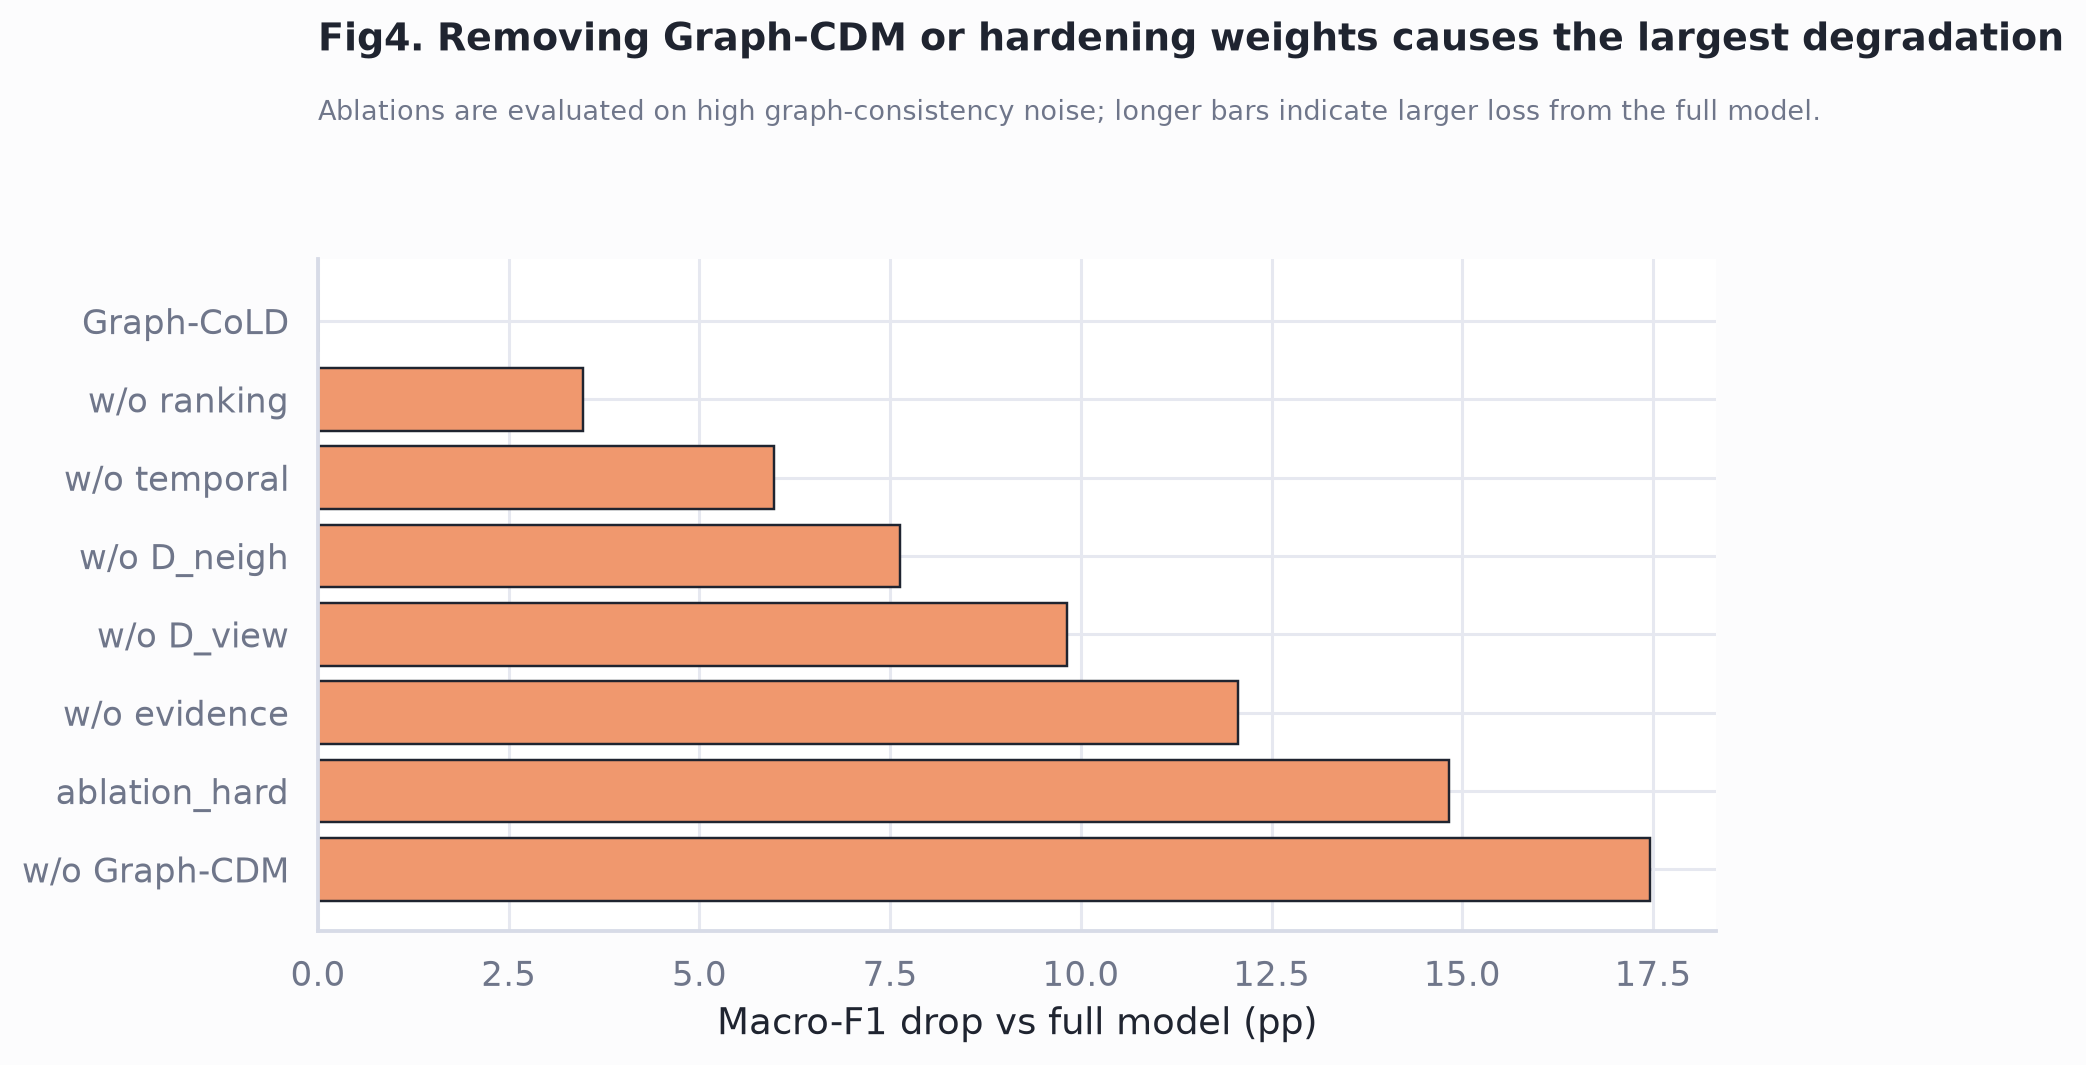
\includegraphics[width=\columnwidth]{fig4_ablation_drop_bar.png}
\caption{Ablation drop comparison.}
\label{fig:ablation}
\end{figure}

\begin{table}[t]
\centering
\caption{SOC emulation results from D6 Table 3.}
\label{tab:optc}
\resizebox{\columnwidth}{!}{%
\begin{tabular}{lrrrr}
\hline
Method & Macro-F1 & ERR & Compression & Top-K\\
\hline
Graph-CoLD & 100.0\% & 90.0\% & 20.0\% & 100.0\%\\
CoLD & 85.1\% & 87.8\% & 23.4\% & 100.0\%\\
Flash & 82.3\% & 86.0\% & 26.0\% & 100.0\%\\
Argus & 82.3\% & 86.2\% & 25.6\% & 100.0\%\\
\hline
\end{tabular}}
\end{table}

\begin{figure}[t]
\centering
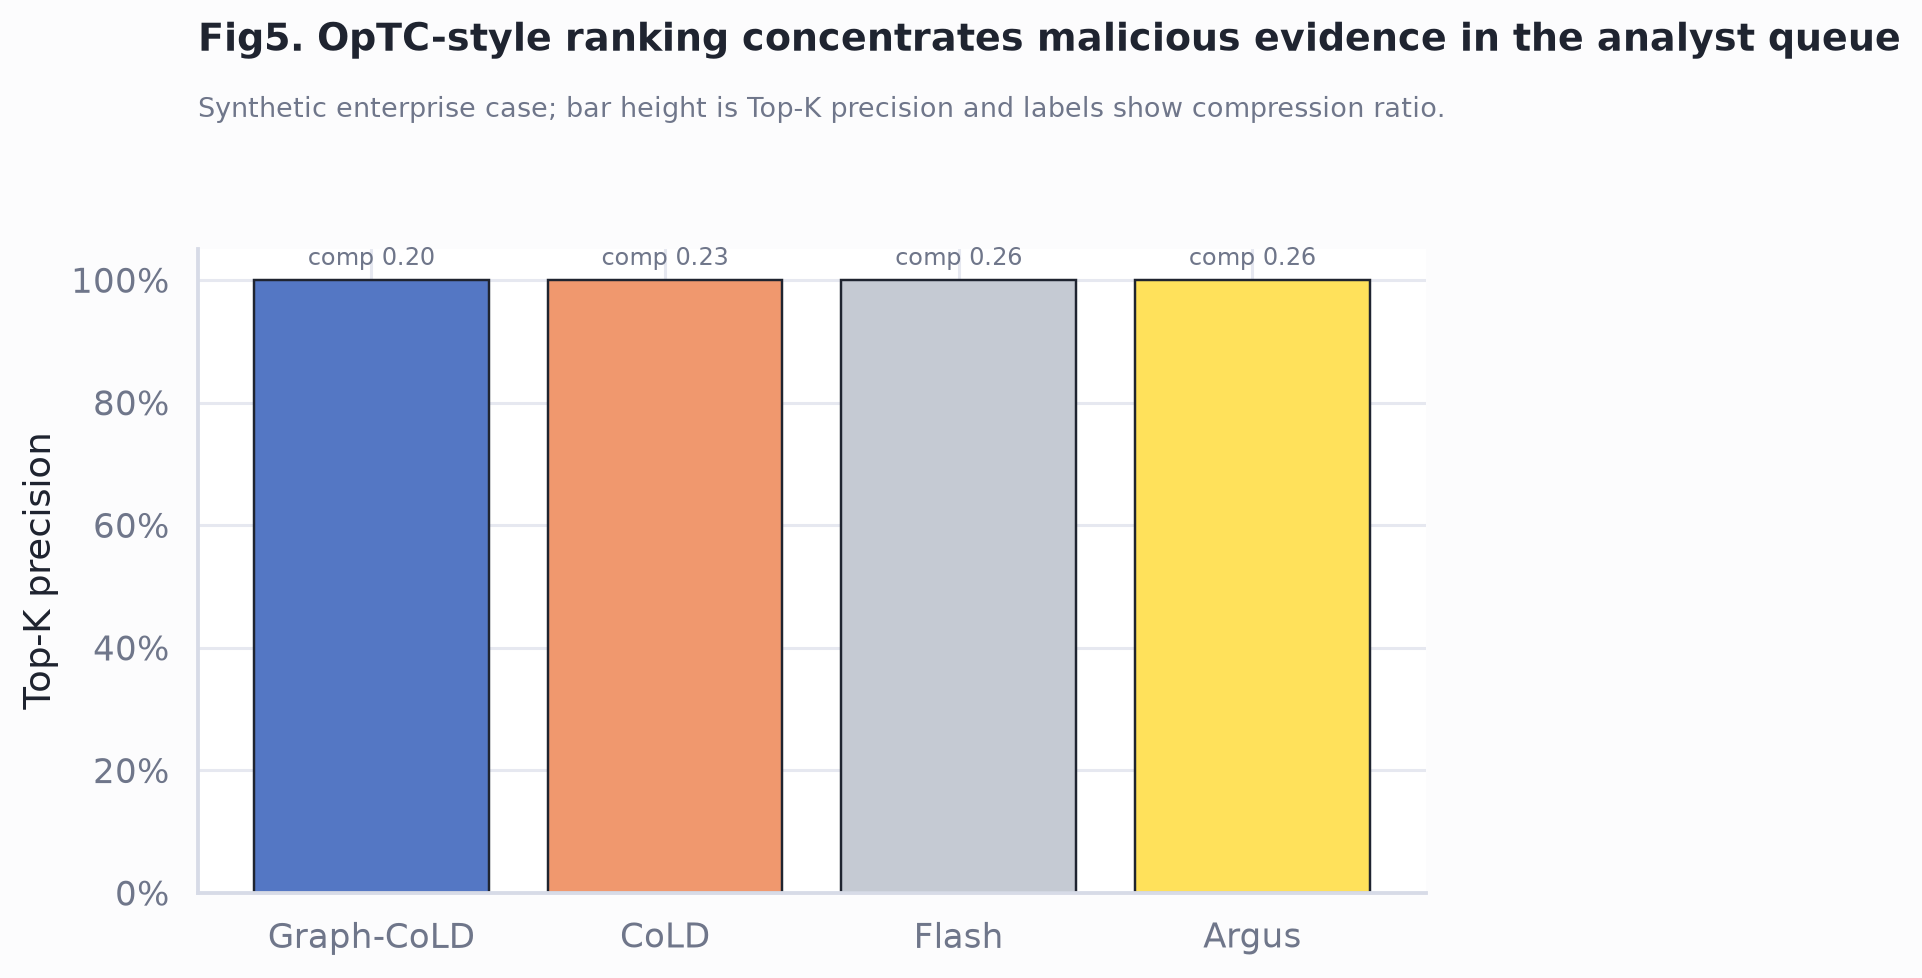
\includegraphics[width=\columnwidth]{fig5_optc_soc_ranking.png}
\caption{SOC ranking in the deterministic enterprise emulation case.}
\label{fig:optc}
\end{figure}

\section{Discussion}
The package preserves D5 synthetic fallback caveats for CICIDS-2017 and MALTLS-22 when raw local datasets are unavailable. The current draft is therefore a reproducible submission package whose empirical claims should be refreshed for final real-data runs. Operationally, Graph-CoLD improves the compression-detection tradeoff by retaining evidence-supported samples rather than applying pure hard deletion. ERR and Tail-ERR complement Macro-F1 by measuring whether the retained queue preserves malicious evidence.

\section{Conclusion}
Graph-CoLD combines multi-view SOC graph representation, Graph-CDM label-space diagnostics, evidence-preserving weighting, and SOC ranking. The D5/D6 outputs show consistent improvements under noisy conditions and practical alert-compression benefits. The package provides an Elsevier Computers \& Security manuscript, an IEEE two-column backup version, and a reproducible build path.

\bibliographystyle{plain}
\bibliography{refs}

\end{document}
